\chapter{Переход от формы вход-выход к форме вход-состояние-выход}
\label{ch:chap2}

\ExplSyntaxOn
\clist_new:N \l_feq_vector_clist
\NewDocumentCommand{\feqvector}{O{\\}mO{b}}{
  \clist_set:Nn \l_feq_vector_clist {#2} % Set the list
  \begin{#3matrix}
  \clist_use:Nn \l_feq_vector_clist {#1} % show it with separator from #1 (\\)
  \end{#3matrix}
}
\ExplSyntaxOff


\definecolor{codegreen}{rgb}{0,0.6,0}
\definecolor{codegray}{rgb}{0.5,0.5,0.5}
\definecolor{codepurple}{rgb}{0.58,0,0.82}
\definecolor{backcolour}{rgb}{0.95,0.95,0.92}

\lstdefinestyle{mystyle}{
    backgroundcolor=\color{backcolour},   
    commentstyle=\color{codegreen},
    keywordstyle=\color{magenta},
    numberstyle=\tiny\color{codegray},
    stringstyle=\color{codepurple},
    basicstyle=\ttfamily\footnotesize,
    breakatwhitespace=false,         
    breaklines=true,                 
    captionpos=b,                    
    keepspaces=true,                 
    numbers=left,                    
    numbersep=5pt,                  
    showspaces=false,                
    showstringspaces=false,
    showtabs=false,                  
    tabsize=2
}
\lstset{style=mystyle}


% \begin{figure}[!ht]
% 	\centering
% \hspace*{\fill}%
% 	\begin{subfigure}[b]{0.49\textwidth}
%         \centering
% 		\includegraphics[width=1\textwidth]{2_18.png}
% 	\end{subfigure}
% \hfill
% 	\begin{subfigure}[b]{0.49\textwidth}
%         \centering
% 		\includegraphics[width=1\textwidth]{2_19.png}
% 	\end{subfigure}
%     \caption{Функция и её сэмплированный вариант}
% \end{figure}
\section{Получение передаточной функции}
Выполним некоторые преобразования:
$$
\begin{aligned}
    \dddot{y} + 6\ddot{y} + 11\dot{y} + 6y = 6\ddot{u} + 4\dot{u} + 16u \\
	(p^3 + 6p^2 + 11p + 6)[y] = (6p^2 + 4p + 16)[u] \\
	y = \frac{6p^2 + 4p + 16}{p^3 + 6p^2 + 11p + 6}[u] + 0
\end{aligned}
$$


В нашем случае передаточная функция $W(p)$ будет выглядеть следующим образом:
$$
W(p) = \frac{6p^2 + 4p + 16}{p^3 + 6p^2 + 11p + 6}
$$
\section{Математические модели}

Чтобы перейти В-В $\rightarrow$ В-C-В в канонической управляемой и наблюдаемой форме, нужно использовать следующие формулы:
\begin{itemize}
  \item Каноническая управляемая форма:
  $$
  \feqvector{\dot{x_1}, \dot{x_2}, \dot{x_3}} = 
	\begin{bmatrix}
		0 & 1 & 0  \\
		0 & 0 & 1 \\
		-a_0 & -a_1 & -a_2
		\end{bmatrix}
	\feqvector{x_1, x_2, x_3} + \feqvector{0, 0, 1}u
  $$

  $$
  y = \feqvector[&]{b_0, b_1, b_2}\feqvector{x_1, x_2, x_3}
  $$

  \item Каноническая наблюдаемая форма:
  $$
  \feqvector{\dot{x_1}, \dot{x_2}, \dot{x_3}} = 
  \begin{bmatrix}
	  0 & 0 & -a_0  \\
	  1 & 0 & -a_1 \\
	  0 & 1 & -a_2
	  \end{bmatrix}
  \feqvector{x_1, x_2, x_3} + \feqvector{b_0, b_1, b_2}u
  $$
  
  $$
  y = \feqvector[&]{0, 0, 1}\feqvector{x_1, x_2, x_3}
  $$

\end{itemize}

Получим следующие результаты:

\begin{itemize}
	\item Каноническая управляемая форма:
	$$
	\feqvector{\dot{x_1}, \dot{x_2}, \dot{x_3}} = 
	  \begin{bmatrix}
		  0 & 1 & 0  \\
		  0 & 0 & 1 \\
		  -6 & -11 & -6
		  \end{bmatrix}
	  \feqvector{x_1, x_2, x_3} + \feqvector{0, 0, 1}u
	$$
  
	$$
	y = \feqvector[&]{16, 4, 6}\feqvector{x_1, x_2, x_3}
	$$
  
	\item Каноническая наблюдаемая форма:
	$$
	\feqvector{\dot{x_1}, \dot{x_2}, \dot{x_3}} = 
	\begin{bmatrix}
		0 & 0 & -6  \\
		1 & 0 & -11 \\
		0 & 1 & -6
		\end{bmatrix}
	\feqvector{x_1, x_2, x_3} + \feqvector{16, 4, 6}u
	$$
	
	$$
	y = \feqvector[&]{0, 0, 1}\feqvector{x_1, x_2, x_3}
	$$
  
  \end{itemize}

Для того, чтобы построить математическую модель В-С-В в диагональной форме, нам нужно будет посмотреть на ПФ, как на дробно-рациональную функцию, а после представить её в виде простейших дробей(такой же приём мы использовали при интегрировании):
$$
W(p) = \frac{6p^2 + 4p + 16}{p^3 + 6p^2 + 11p + 6} = -\frac{32}{p+2} + \frac{29}{p+3} + \frac{9}{p+1} = -\frac{8\cdot 4}{p+2} + \frac{29\cdot 1}{p+3} + \frac{3\cdot 3}{p+1} 
$$
$$
W(p) = -\frac{8\cdot 4}{p+2} + \frac{29\cdot 1}{p+3} + \frac{3\cdot 3}{p+1} = \frac{\beta_1\cdot \gamma_1}{p-\lambda_1} + \frac{\beta_2 \cdot \gamma_2}{p-\lambda_2} + \frac{\beta_3\cdot \gamma_3}{p-\lambda_3}
$$
\begin{itemize}
	\item Диагональная форма:
	$$
	\feqvector{\dot{x_1}, \dot{x_2}, \dot{x_3}} = 
	  \begin{bmatrix}
		  \lambda_1 & 0 & 0  \\
		  0 & \lambda_2 & 0 \\
		  0 & 0 & \lambda_3
		  \end{bmatrix}
	  \feqvector{x_1, x_2, x_3} + \feqvector{\beta_1, \beta_2, \beta_3}u
	$$
  
	$$
	y = \feqvector[&]{\gamma_1, \gamma_2, \gamma_3}\feqvector{x_1, x_2, x_3}
	$$
	\item С моими коэффициентами:
	$$
	\feqvector{\dot{x_1}, \dot{x_2}, \dot{x_3}} = 
	  \begin{bmatrix}
		  -2 & 0 & 0  \\
		  0 & -3 & 0 \\
		  0 & 0 & -1
		  \end{bmatrix}
	  \feqvector{x_1, x_2, x_3} + \feqvector{-8, 29, 3}u
	$$
  
	$$
	y = \feqvector[&]{4, 1, 3}\feqvector{x_1, x_2, x_3}
	$$
  \end{itemize}

\section{Моделирование полученных форм}
Составим схемы с учётом того, что должны быть видны чётко каналы, соответствующие компонентам векторов состояния $x$:

\begin{figure}[ht]
    \centering
    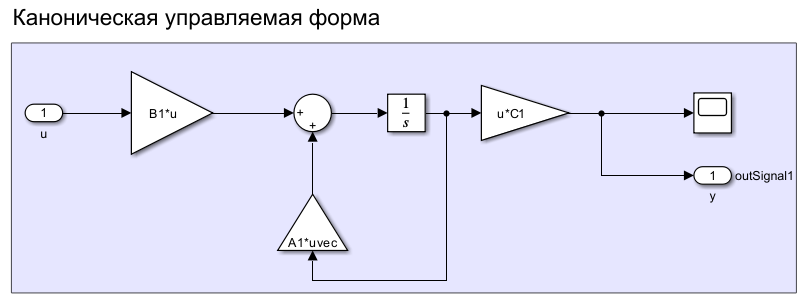
\includegraphics[width=1\textwidth]{scheme_task2_controlled.png}
	\caption{Схема системы - управляемая форма}
\end{figure}
\begin{figure}[ht]
    \centering
    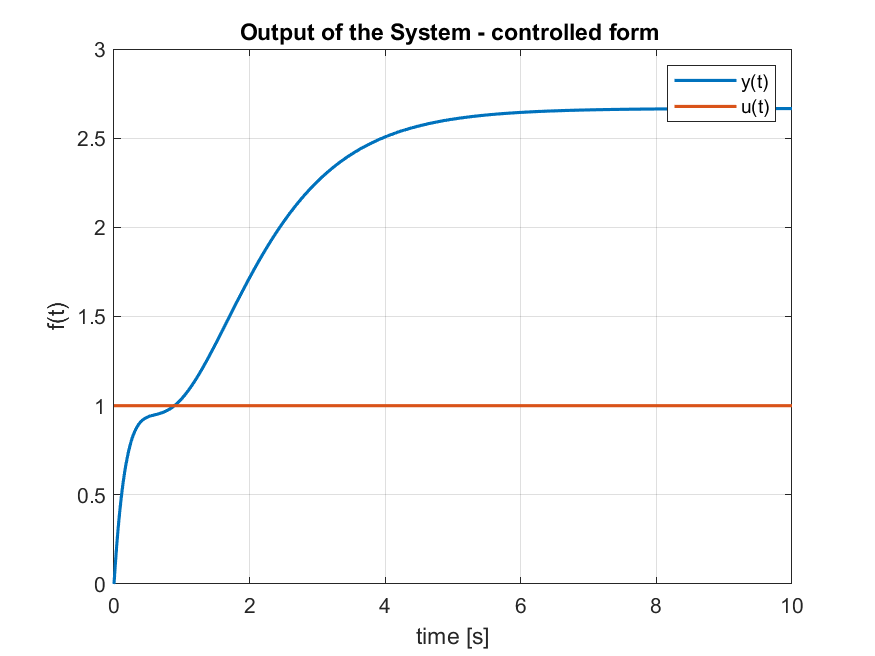
\includegraphics[width=0.5\textwidth]{output_task2_controlled.png}
	\caption{Симуляция - управляемая форма}
\end{figure}

\newpage
\begin{figure}[ht]
    \centering
    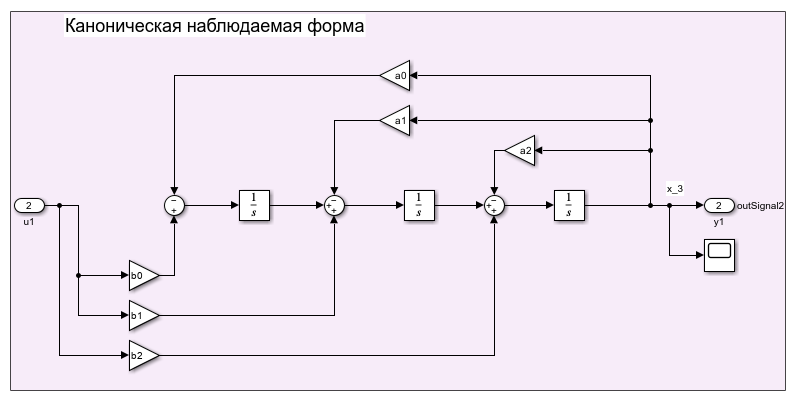
\includegraphics[width=1\textwidth]{scheme_task2_observable.png}
	\caption{Схема системы - наблюдаемая форма}
\end{figure}
\begin{figure}[ht]
    \centering
    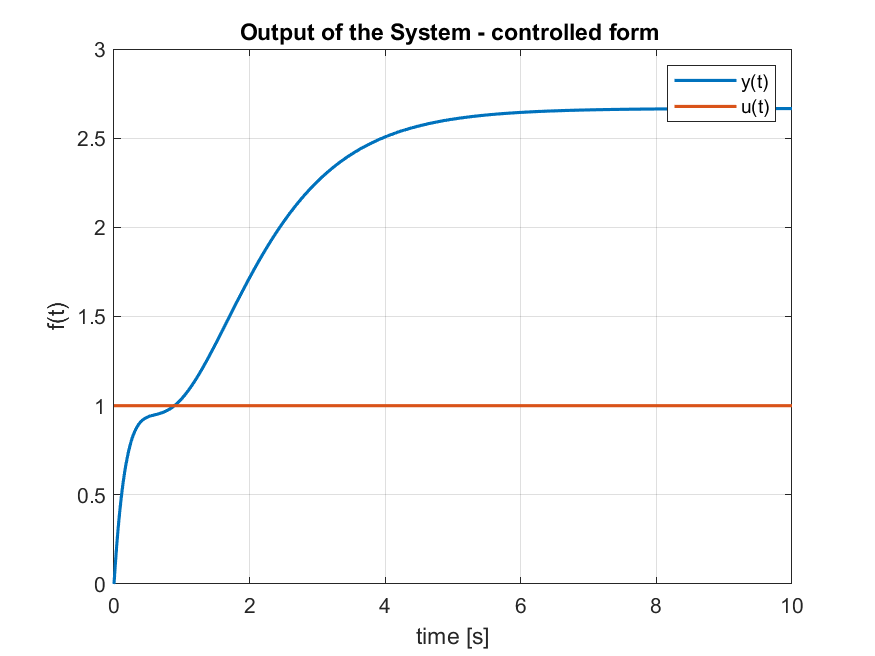
\includegraphics[width=0.5\textwidth]{output_task2_controlled.png}
	\caption{Симуляция - наблюдаемая форма}
\end{figure}

\newpage
\begin{figure}[ht] 
    \centering
    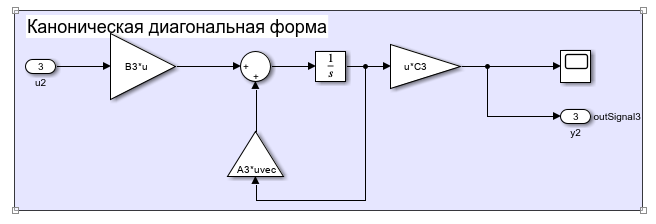
\includegraphics[width=1\textwidth]{scheme_task2_diagonal.png}
	\caption{Схема системы - диагональная форма}
\end{figure}
\begin{figure}[ht]
    \centering
    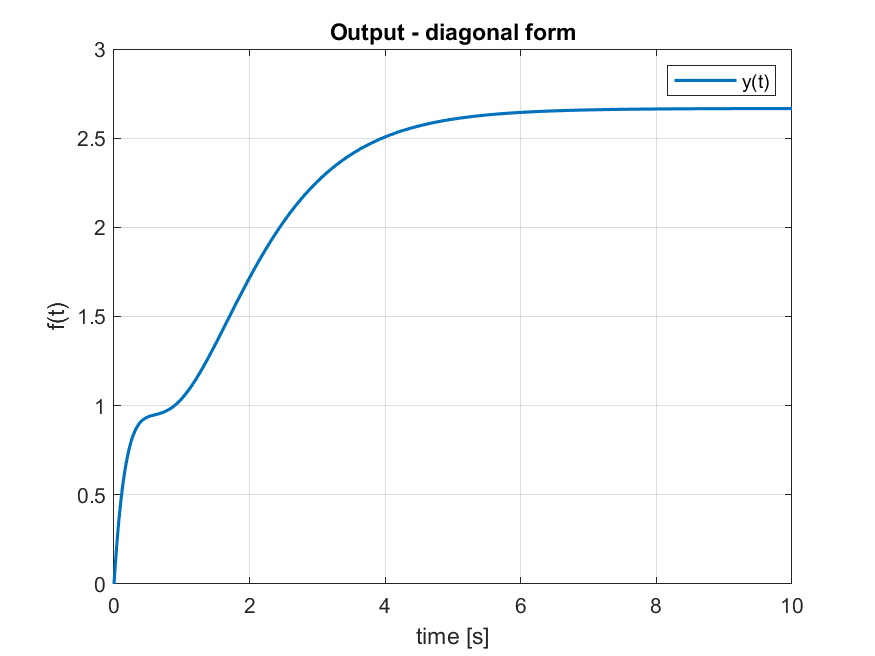
\includegraphics[width=0.5\textwidth]{output_task2_diagonal.png}
	\caption{Симуляция - диагональная форма}
\end{figure}

\section{Выводы}

Невооружённым взглядом видно, что все графики вышли идентичными между собой и по сравнению с формой В-В.

Несложно понять почему это так - ведь мы меняем только вид схемы, меняем точку зрения на систему.

\endinput